\subsection{Pasos a nivel}

    % Autoridad > derecho limitado a una porcion
    % Claridad > autoridad no ambigua
    % Anticipacion > avisar con antelacion
    % Granularidad > rutas cortas y funcionales
    % Terminalidad > avisar fin de via
    % Infraestructura > avisar de infraestructura
    % No bloqueo > circulacion fluida
    
    En la Sección \ref{sec:crossing} definimos la clase levelCrossing que modela a los cruces ferroviarios a nivel. Los cruces ferroviarios son un sector crítico de los sistemas ferroviarios ya que conviven tanto las formaciones como los vehículos y peatones. El cruce ferroviario impone un límite a la autoridad ya que es necesario confirmar que la barrera ferroviaria se encuentre baja antes de habilitar a una formación. Además, podemos utilizar al cruce ferroviario como frontera entre dos rutas, aplicando el principio de granuralidad ($P_4$). Esto se refuerza con el principio de infraestructura ($P_6$) ya que, aún cuando la formación no puede dañar la barrera ferroviaria al transitar el paso a nivel sin autoridad, puede dañar severamente a los conductores de vehículos o peatones.

    Por el principio de anticipación ($P_3$), las señales se colocan a varios metros de distancia del cruce ferroviario. Las barreras ferroviarias comienzan su descenso al detectar la presencia de una formación bastantes metros antes de estas señales. De esta manera la formación llegará el cruce ferroviario cuando las barreras ya han descendido. De igual forma, las barreras ferroviarias suelen complementarse con indicaciones lumínicas y sonoras que se activan al comienzo del descenso. Para asegurar una circulación fluida, por el principio de granuralidad ($P_4$), las formaciones deberán tener una mayor prioridad que los vehículos y peatones, haciendo descender la barrera siempre que una formación se aproxime, sin excepciones.

    En el Algoritmo \ref{alg:LC} definimos a la señal de circulación como la única señal necesaria para operar un cruce ferroviario, protegiendo a todos los vehículos, peatones y formaciones que quieran hacer uso de la intersección. En el caso de que la vía se bidireccional se añadirán señales de circulación para proteger el cruce en ambos sentidos.

    \begin{algorithm}[hbt!]
        \caption{Algoritmo de generación de señalamiento para levelCrossing.}\label{alg:LC}
        \DontPrintSemicolon
        %\SetAlgoLined
        \SetNoFillComment
        \LinesNotNumbered 
        \For { netElement WITH LevelCrossing }
        {
            \tcc{Before reaching level crossing}
            [Signals] $\gets$ ADD circulation signal $\gg\gg$\;
            \tcc{After leaving level crossing}
            [Signals] $\gets$ ADD circulation signal $\ll\ll$\;
        }
        \KwResult{[Signals]} 
    \end{algorithm}    
    
    Aplicando el Algoritmo \ref{alg:LC} a un sistema de dos vías paralelas con un cruce de ferroviario que atraviese perpendicularmente ambas vías obtenemos el resultado ilustrado en la Figura \ref{fig:signal_crossing}. Se asumieron que ambas vías son bidireccionales, en caso contrario solo se generarían las señales S01 y S02.
    
    \begin{figure}[h!]
        \centering
        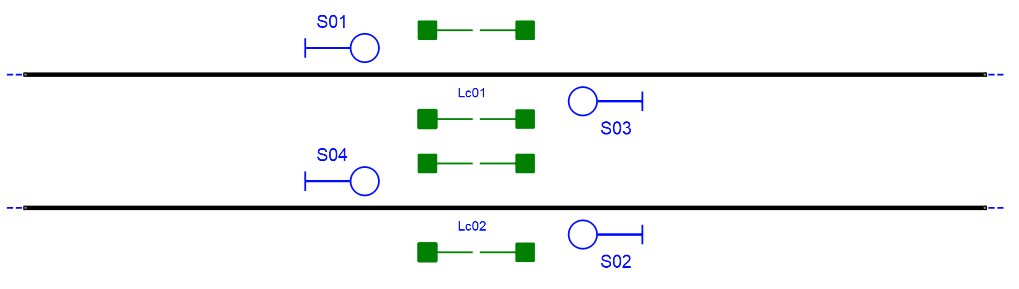
\includegraphics[width=1\textwidth]{Figuras/crossings.PNG}
        \centering\caption{Señalamiento generado para cruces ferroviarios.}
        \label{fig:signal_crossing}
    \end{figure}
    
    Una formación que circule de izquierda a derecha deberá detenerse antes de la señal S01, en caso de utilizar la vía superior, o antes de la señal S04, en caso de utilizar la vía inferior. Las señales presentarán un aspecto rojo si las barreras se encuentren altas o en proceso de descender. Análogamente, las formaciones deberán detenerse antes de las señales S03 y S02 en el caso de transitar de derecha a izquierda por la vía superior o inferior respectivamente. Cuando las barreras se encuentren bajas, los aspectos de las señales cambiarán a verde para habilitar la circulación de la formación por sobre el paso a nivel, continuando su marcha hasta la próxima señal disponible, fuera del alcance de lo ilustrado en la Figura \ref{fig:signal_crossing}.    